\documentclass[11pt,a4paper]{article}
\usepackage[utf8]{inputenc}
\usepackage[T1]{fontenc}
\usepackage{babel}
\babelprovide[import=pt-BR,main]{brazilian}
\usepackage{lmodern,microtype}
\usepackage{amsmath,amssymb,graphicx,booktabs,array}
\usepackage[margin=2.2cm,headheight=15pt]{geometry}
\usepackage{xcolor,fancyhdr,caption,hyperref}
\definecolor{azul}{HTML}{173D58}
\hypersetup{colorlinks=true,linkcolor=azul,urlcolor=azul,
 pdftitle={Autoconvergência da Equação do Telegrafista: resumo expandido},
 pdfsubject={Resultados numéricos para discussão no TCC}}
\captionsetup{font=small,labelfont=bf}
\pagestyle{fancy}
\fancyhf{}
\fancyhead[L]{\small\color{azul} Equação do Telegrafista | Autoconvergência}
\fancyhead[R]{\small TCC}
\fancyfoot[C]{\small\thepage}
\setlength{\parindent}{1.1em}
\setlength{\parskip}{3pt}
\setlength{\emergencystretch}{2em}
\newcommand{\secao}[1]{\section{\texorpdfstring{\color{azul}#1}{#1}}}
\newcommand{\arquivo}[1]{\texttt{\detokenize{#1}}}
\begin{document}
\thispagestyle{empty}
\begin{center}
{\small\color{azul} RESUMO EXPANDIDO DE RESULTADOS}\par\medskip
{\LARGE\bfseries\color{azul} Autoconvergência da Equação\\[3pt] do Telegrafista em uma dimensão}\par\medskip
{\large Experimento combinado com amortecimento e reação}\par\smallskip
{\small Material para discussão com a orientação do TCC | 1 de outubro de 2026}
\end{center}
\vspace{2mm}
\noindent\textbf{Resumo.} Apresenta-se um estudo reproduzível de autoconvergência
da Equação do Telegrafista, utilizando a implementação Classic Clawpack existente
no projeto. Foram executadas sete malhas uniformes, de 32 a 2048 células físicas,
para uma condição inicial gaussiana e parâmetros fixos de amortecimento e reação.
As soluções em $t=0{,}8$ foram comparadas por restrição conservativa da malha fina
à grossa, calculando-se erros de refinamento e ordens observadas para $u$ e $u_t$.
As diferenças de $u$ diminuem em todos os pares, enquanto $u_t$ apresenta
comportamento não monotônico nas primeiras malhas. Na última trinca disponível,
as ordens locais são $p_u\approx0{,}8454$ e $p_{u_t}\approx2{,}1573$.
O estudo avalia o esquema completo, incluindo a integração da fonte e a evolução
temporal; não permite atribuir uma ordem única ao método nem isolar o erro espacial.
\par\smallskip
\noindent\textbf{Palavras-chave:} Equação do Telegrafista; volumes finitos;
Clawpack; autoconvergência; refinamento de malha.

\secao{Objetivo e modelo implementado}
O objetivo é verificar como as soluções numéricas se modificam sob refinamentos
sucessivos, seguindo a referência metodológica fornecida pela orientadora [1].
Considera-se
\begin{equation}
 u_{tt}+a\,u_t=c^2u_{xx}+b\,u,\qquad x\in[-2,2],\quad 0\leq t\leq0{,}8.
\end{equation}
A inspeção dos fontes confirmou $q_1=u$, $q_2=u_t$ e $q_3=u_x$, com
sinal positivo no termo $b\,u$. A formulação de primeira ordem é
\begin{equation}
 (q_1)_t=q_2,\qquad (q_2)_t-c^2(q_3)_x=bq_1-aq_2,
 \qquad (q_3)_t-(q_2)_x=0.
\end{equation}
Foram fixados $c=2$, $a=1$, $b=1$, $\beta=200$ e $x_0=0$, com
\begin{equation}
 u(x,0)=e^{-\beta(x-x_0)^2},\quad u_t(x,0)=0,\quad
 u_x(x,0)=-2\beta(x-x_0)e^{-\beta(x-x_0)^2}.
\end{equation}
A inicialização existente avalia essas expressões nos centros das células e foi
preservada. O parâmetro $b=1$ representa reação com sinal positivo na equação;
não deve ser confundido com a configuração $b=-1$ de outros casos do projeto.

\secao{Configuração numérica preservada}
A parte hiperbólica utiliza correção de segunda ordem e limitadores MC. A fonte
permanece ativa, com separação de Godunov (\arquivo{source_split=1}) e Euler
explícito simultâneo: $q_1^+=q_1+\Delta t\,q_2$ e
$q_2^+=q_2+\Delta t(bq_1-aq_2)$, usando os valores anteriores à etapa da fonte.
O passo é variável, a CFL desejada é $0{,}9$ e a máxima permitida é $1$.
Mantiveram-se os contornos por extrapolação e 64 intervalos de saída, além do
estado inicial. Não houve alteração do solver, dos limitadores ou da fonte.

\newpage
\secao{Comparação conservativa e cálculo das ordens}
Executaram-se somente
\[
 N\in\{32,64,128,256,512,1024,2048\},\qquad \Delta x=\frac{4}{N}.
\]
Aqui, $N$ conta \textbf{células físicas}, não vértices. As saídas ASCII do Classic
contêm exatamente $N$ registros físicos; células fantasma não entram nas somas.
A componente $u_t$ é lida diretamente de $q_2$, sem aproximação por diferenças
entre tempos de saída. Todas as comparações usam o tempo efetivamente registrado
nos arquivos: $t=0{,}7999999999999992$, compatível com $0{,}8$ à tolerância
de $10^{-11}$.

As soluções de volumes finitos são tratadas como aproximações de médias
celulares. A avaliação inicial no centro não muda essa interpretação. Como as
fronteiras das células coincidem e a razão de refinamento é dois, aplica-se,
separadamente a cada componente,
\begin{equation}
 (R v^{2N})_i=\frac{v^{2N}_{2i-1}+v^{2N}_{2i}}{2},\qquad i=1,\ldots,N.
\end{equation}
Essa média reúne duas células finas no mesmo volume da célula grossa; não se
seleciona apenas um valor a cada dois. Para $v=u$ ou $v=u_t$, definem-se
\begin{equation}
 E_v(N)=\left[\frac1N\sum_{i=1}^N
       \big((Rv^{2N})_i-v^N_i\big)^2\right]^{1/2},\qquad
 p_v(N)=\frac{\log\big(E_v(N)/E_v(2N)\big)}{\log2}.
\end{equation}
$E_v$ é o \textbf{erro $L^2$ discreto normalizado entre malhas}, ou erro de
refinamento. Não é erro contra uma solução exata nem desvio padrão:
não se subtrai a média e não se divide por $N-1$.

Uma ordem exige três soluções: $N$, $2N$ e $4N$. Na Tabela~\ref{tab:resultados},
a linha $N$ contém $E(N)$ e $p(N)$; essa organização difere da tabela ilustrativa
da referência [1], que coloca $E(N)$ na linha $2N$. A adaptação por restrição
conservativa também explicita a interpretação de volumes finitos, em lugar
de comparação pontual por interpolação.

\begin{table}[h!]
\centering
\caption{Resultados calculados em $t=0{,}8$. Cada erro usa o par $N\to2N$;
cada ordem usa a trinca $N\to2N\to4N$.}
\label{tab:resultados}
\small\setlength{\tabcolsep}{4pt}\renewcommand{\arraystretch}{1.22}
\begin{tabular}{rrrrrr}
\toprule
$N$ & $\Delta x$ & $E_u(N)$ & $p_u(N)$ & $E_{u_t}(N)$ & $p_{u_t}(N)$\\
\midrule
32 & 0{,}125 & $7{,}441192\times 10^{-2}$ & 1{,}2388 & $2{,}466716\times 10^{-1}$ & -1{,}9362 \\
64 & 0{,}0625 & $3{,}153010\times 10^{-2}$ & 1{,}1962 & $9{,}439708\times 10^{-1}$ & 0{,}4824 \\
128 & 0{,}03125 & $1{,}376038\times 10^{-2}$ & 1{,}6681 & $6{,}756928\times 10^{-1}$ & 1{,}4129 \\
256 & 0{,}015625 & $4{,}329820\times 10^{-3}$ & 1{,}5398 & $2{,}537534\times 10^{-1}$ & 2{,}0576 \\
512 & 0{,}0078125 & $1{,}489155\times 10^{-3}$ & 0{,}8454 & $6{,}095455\times 10^{-2}$ & 2{,}1573 \\
1024 & 0{,}00390625 & $8{,}288204\times 10^{-4}$ & -- & $1{,}366411\times 10^{-2}$ & -- \\
2048 & 0{,}001953125 & -- & -- & -- & -- \\
\bottomrule

\end{tabular}
\end{table}
\noindent\small São seis erros e cinco ordens por componente. Os traços indicam
valores indisponíveis, registrados como \arquivo{NaN} no CSV: $E(2048)$,
$p(1024)$ e $p(2048)$. Não foram preenchidos com zero.\normalsize

\medskip
Para $u$, as diferenças diminuem em todos os pares. Para $u_t$, o erro entre
64 e 128 células é maior que entre 32 e 64; por isso a primeira ordem é
negativa. Os dados das malhas grossas não sustentam uma taxa assintótica.

\newpage
\secao{Erros de refinamento e passos temporais}
\begin{figure}[h!]
\centering
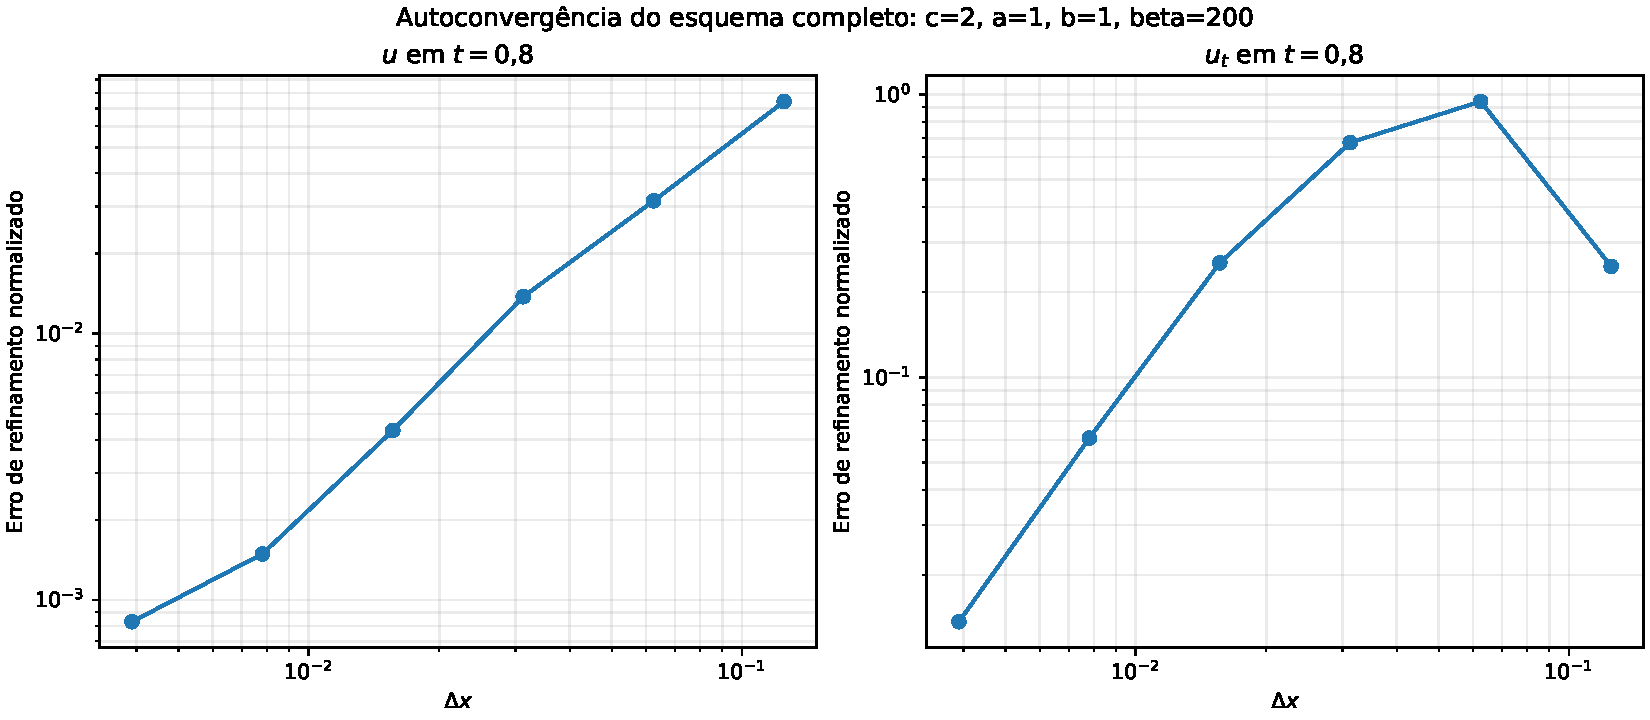
\includegraphics[width=\linewidth]{figuras/erros_loglog.pdf}
\caption{Erros calculados em função de $\Delta x$, em escala log-log.
O refinamento corresponde à redução de $\Delta x$. A inversão nas malhas
grossas de $u_t$ está preservada. Fonte: saídas deste experimento.}
\label{fig:erros}
\end{figure}

\begin{table}[h!]
\centering
\caption{Diagnóstico das execuções: passos aceitos, tentativas rejeitadas,
intervalos de CFL efetiva e máximo inicial amostrado de $u$.}
\label{tab:passos}
\small\renewcommand{\arraystretch}{1.16}
\begin{tabular}{rrrrr}
\toprule
$N$ & Aceitos & Rejeitadas & CFL efetiva (mín.--máx.) & $\max_i u_i(0)$\\
\midrule
32 & 64 & 0 & $0{,}200$--$0{,}200$ & $0{,}457833$\\
64 & 64 & 0 & $0{,}400$--$0{,}400$ & $0{,}822578$\\
128 & 64 & 0 & $0{,}800$--$0{,}800$ & $0{,}952345$\\
256 & 128 & 1 & $0{,}700$--$0{,}900$ & $0{,}987867$\\
512 & 256 & 1 & $0{,}500$--$0{,}900$ & $0{,}996953$\\
1024 & 512 & 1 & $0{,}100$--$0{,}900$ & $0{,}999237$\\
2048 & 960 & 1 & $0{,}200$--$0{,}900$ & $0{,}999809$\\
\bottomrule
\end{tabular}
\end{table}

A CFL \emph{desejada} é $0{,}9$, mas a CFL \emph{efetiva} depende dos passos
aceitos. Nas malhas $N=32,64,128$, o intervalo de saída $0{,}8/64=0{,}0125$
limita o passo: todas usam $\Delta t=0{,}0125$, apesar dos refinamentos espaciais.
Nas demais malhas, os passos também são ajustados para alcançar os tempos de
saída. Portanto, o estudo acopla refinamento espacial e temporal sem manter uma
CFL única em todos os passos.

Os diagnósticos foram extraídos dos passos aceitos no log, excluindo as
tentativas rejeitadas. O registro de CFL tem três casas decimais; $\Delta t$
e $t$ no log têm cinco algarismos significativos. São valores arredondados.
Os campos de \arquivo{fort.info} incluem candidatos ao próximo passo e o
passo inicial configurado; não foram confundidos com os passos usados.
A opção de registro \arquivo{verbosity=1} foi a única mudança de configuração
voltada ao diagnóstico e não altera o algoritmo numérico.

A largura à meia altura da gaussiana é
$2\sqrt{\log(2)/200}\approx0{,}117741$. Em $N=32$, $\Delta x=0{,}125$
supera essa largura e $x_0=0$ fica entre centros. A resolução inicial insuficiente,
evidenciada pelos máximos da Tabela~\ref{tab:passos}, é relevante para
interpretar os resultados grosseiros.

\newpage
\secao{Perfis das soluções no tempo final}
Os gráficos mostram as sete malhas no mesmo tempo físico. Os painéis à direita
ampliam o pulso direito para permitir a inspeção das diferenças locais.

\begin{figure}[h!]
\centering
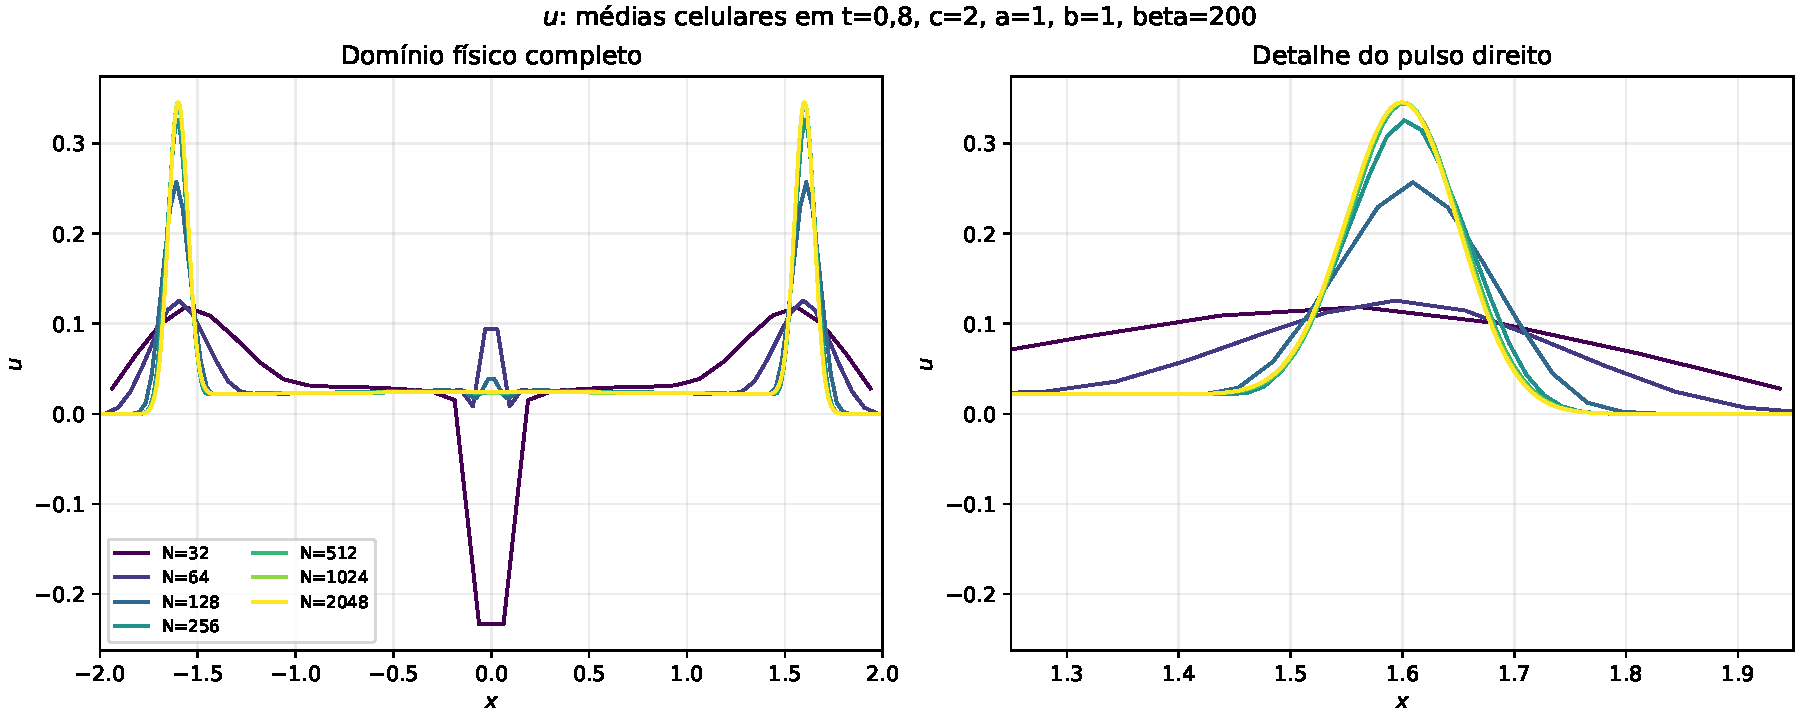
\includegraphics[width=\linewidth]{figuras/perfis_u.pdf}
\caption{Perfis de $u(x,0{,}8)$ no domínio completo e em ampliação.
Em $N=32$ aparecem deformação dos pulsos e uma região central negativa.
Esses resultados foram mantidos para avaliação, sem correções posteriores.
Fonte: saídas deste experimento.}
\label{fig:u}
\end{figure}
\begin{figure}[h!]
\centering
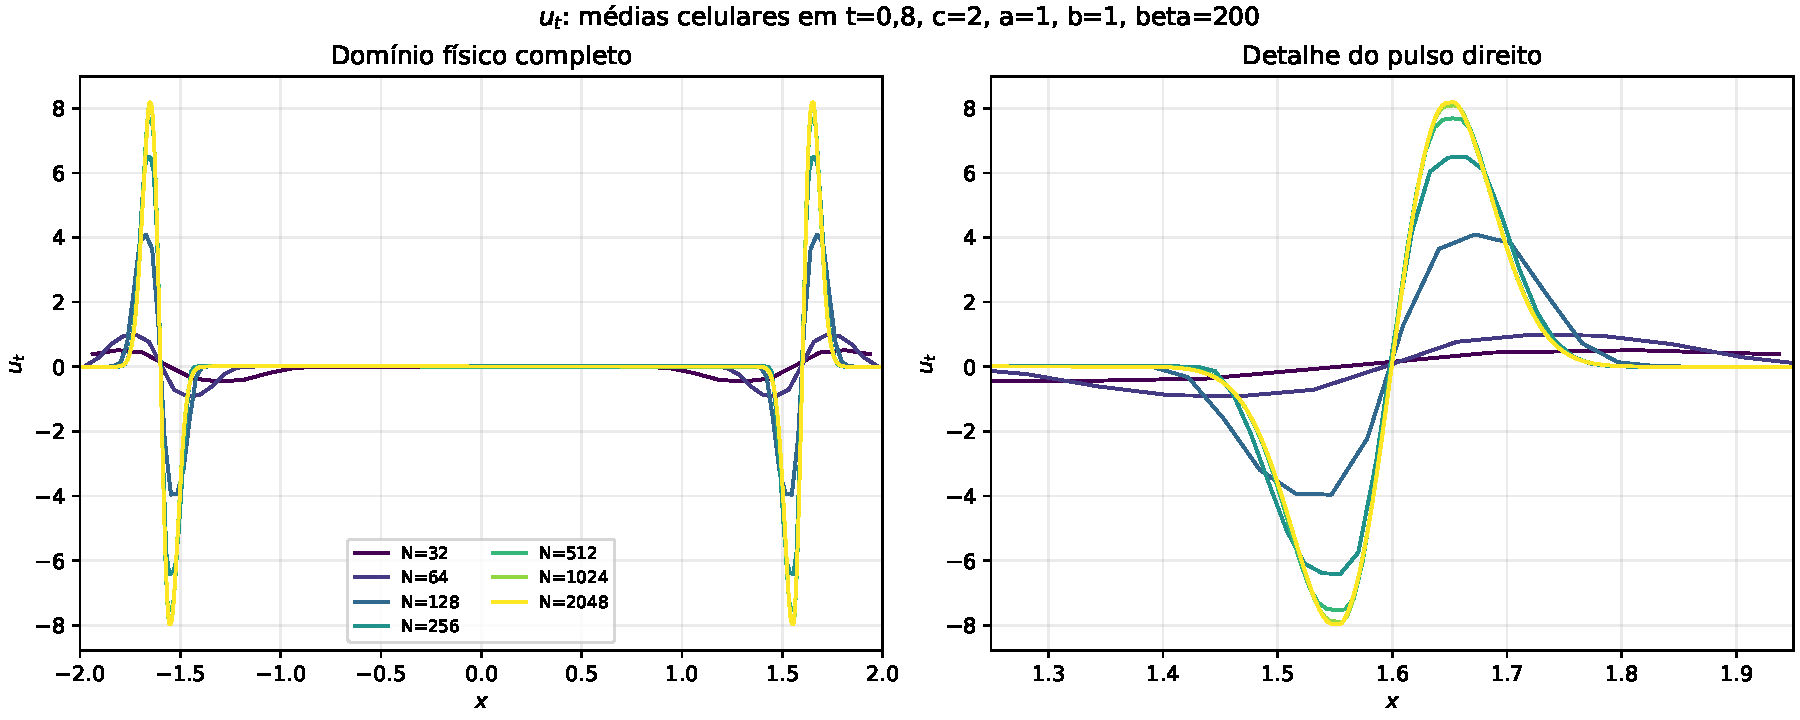
\includegraphics[width=\linewidth]{figuras/perfis_ut.pdf}
\caption{Perfis de $u_t(x,0{,}8)$, obtidos da segunda componente do solver.
As malhas grossas representam de forma muito distinta a estrutura dos pulsos;
as curvas mais finas apresentam maior proximidade.
Fonte: saídas deste experimento.}
\label{fig:ut}
\end{figure}

\noindent A semelhança visual das curvas finas deve ser analisada junto com os
erros integrados: sobreposição no gráfico, por si só, não determina a ordem do
esquema nem demonstra convergência para a solução exata.

\newpage
\secao{Discussão, verificações e conclusão}
Na última trinca $512\to1024\to2048$, obtiveram-se
$p_u=0{,}8454$ e $p_{u_t}=2{,}1573$. As duas últimas ordens de $u_t$
são próximas de dois ($2{,}0576$ e $2{,}1573$), enquanto as de $u$ são
variáveis e a última é inferior a um. Essa diferença entre componentes
impede resumir os resultados como ``o método tem ordem dois''.

A correção hiperbólica é de segunda ordem, mas o splitting de Godunov e
o Euler explícito da fonte são de primeira ordem. Os limitadores e a
inicialização amostrada também integram o cálculo. As ordens observadas
refletem a combinação dessas etapas, da resolução da gaussiana e dos passos
efetivos. Não foi realizado um experimento que isolasse a contribuição de cada
etapa; a origem dos artefatos grosseiros não foi determinada separadamente.
O domínio e os contornos foram mantidos, mas a independência em relação ao
contorno não foi demonstrada.

\noindent\textbf{Verificações numéricas.} As sete execuções terminaram com
código zero e \arquivo{info=0}. Conferiram-se as 455 saídas (65 por malha),
incluindo número de células, geometria, tempos registrados, parâmetros,
finitude e condição inicial. A comparação verifica alinhamento das fronteiras
e razão dois. Uma auditoria independente reproduziu os seis erros e as cinco
ordens por componente. Os resultados e o funcionamento dos Casos 2--8 foram
preservados; não se executou $N=4096$ ou outro conjunto de parâmetros.

\noindent\textbf{Testes sintéticos, separados do solver.} Diferença constante
igual a um produziu erro normalizado um; a restrição preservou dados constantes;
erros reduzidos por fator quatro produziram ordem dois. A suíte de verificação
passou em oito testes. Esses valores verificam rotinas de cálculo e não são
resultados físicos nem evidência de ordem dois para o experimento real.

\noindent\textbf{Conclusão.} O estudo documenta redução das diferenças de $u$
e aproximação dos perfis finos das duas componentes, mas não estabelece uma
ordem global única ou erro contra solução exata. As malhas grossas têm limitações
claras de resolução e de evolução temporal. Os resultados são apresentados
para discussão metodológica com a orientação, sem ajuste do método para
obter uma taxa desejada.

\secao{Automação, proveniência e reprodução}
A automação em \arquivo{autoconvergencia.py} compila os fontes atuais conforme
o Makefile da pasta \arquivo{arquivos-roteiro-simulacoes/}. A compilação ocorre
em diretório próprio. Cada malha possui pasta, parâmetros, log e dados próprios. A instalação
é localizada por \arquivo{CLAW}, \arquivo{--claw} ou pela configuração disponível.
Foram registrados Clawpack 5.14.0, GNU Fortran 16.2.1, opção \arquivo{-O2},
branch \arquivo{tcc-simulacoes} e commit \arquivo{3bab969a11eb}.
A árvore continha alterações não commitadas: hashes e cópias dos fontes
identificam a versão efetivamente executada, além do commit.

Na pasta \arquivo{arquivos-roteiro-simulacoes/}, os comandos são:
\begin{quote}\small\ttfamily
python3 -m unittest -v test\_autoconvergencia.py\\
python3 autoconvergencia.py\\
python3 autoconvergencia.py --somente-analisar
\end{quote}
As saídas, o CSV, as figuras e o relatório estão em
\arquivo{resultados_autoconvergencia/}. O pacote deste resumo inclui os gráficos
vetoriais, o CSV e os registros usados na redação; as saídas brutas permanecem no
repositório. Não há bloqueio de execução registrado. Este material é independente
da monografia e não foi publicado automaticamente.

\medskip\noindent\textbf{Referências e fontes dos dados}\par
\noindent\small [1] \textit{Análise de Erro e Ordem de Convergência}.
Arquivo \arquivo{calculo_erro_ordem.tex}, fornecido pela orientadora; referência
metodológica interna, sem data indicada.\par
\noindent [2] Projeto \textit{clawpack-telegraph\_1d}, branch
\arquivo{tcc-simulacoes}. Fontes da aplicação, \arquivo{autoconvergencia.csv},
\arquivo{RELATORIO.md} e \arquivo{experimento.json} do estudo de autoconvergência.
Clawpack Classic 5.14.0, commit Classic \arquivo{6b3dfe6419d9}.
\end{document}
